%% Unit 2: Basics of Design Thinking
%% Included from main.tex via %% Unit 2: Basics of Design Thinking
%% Included from main.tex via %% Unit 2: Basics of Design Thinking
%% Included from main.tex via %% Unit 2: Basics of Design Thinking
%% Included from main.tex via \include{./units/unit2}
%% Requires the macros/colours defined in main.tex's preamble.

%==============================================================================
\section{Basics of Design Thinking}
%==============================================================================
\unitdivider{II}{Basics of Design Thinking}{The mindset, the process, the tools}

\begin{frame}{What is Design Thinking?}
  \accentrule\\[0.3em]
  \begin{columns}[T]
    \begin{column}{0.55\textwidth}\small
      \begin{block}{Definition}\small
        A \kw{human-centred}, iterative problem-solving approach that seeks
        to understand users, challenge assumptions, redefine problems and
        create innovative solutions to prototype and test.
      \end{block}
      \textbf{Need for design thinking}
      \begin{itemize}\small
        \item Problems are \kwc{complex \& ill-defined}.
        \item Users' real needs are often \emph{hidden}.
        \item Reduces the risk of building the wrong thing.
      \end{itemize}
    \end{column}
    \begin{column}{0.45\textwidth}\small
      \textbf{Objectives}
      \begin{itemize}\small
        \item Keep the \kwt{user at the centre}.
        \item Encourage \kwt{creativity \& collaboration}.
        \item \kwt{Fail early}, learn cheaply.
        \item Turn insight into tangible value.
      \end{itemize}
    \end{column}
  \end{columns}
\end{frame}

\begin{frame}{Concepts \& Brainstorming}
  \begin{columns}[c]
    \begin{column}{0.58\textwidth}
      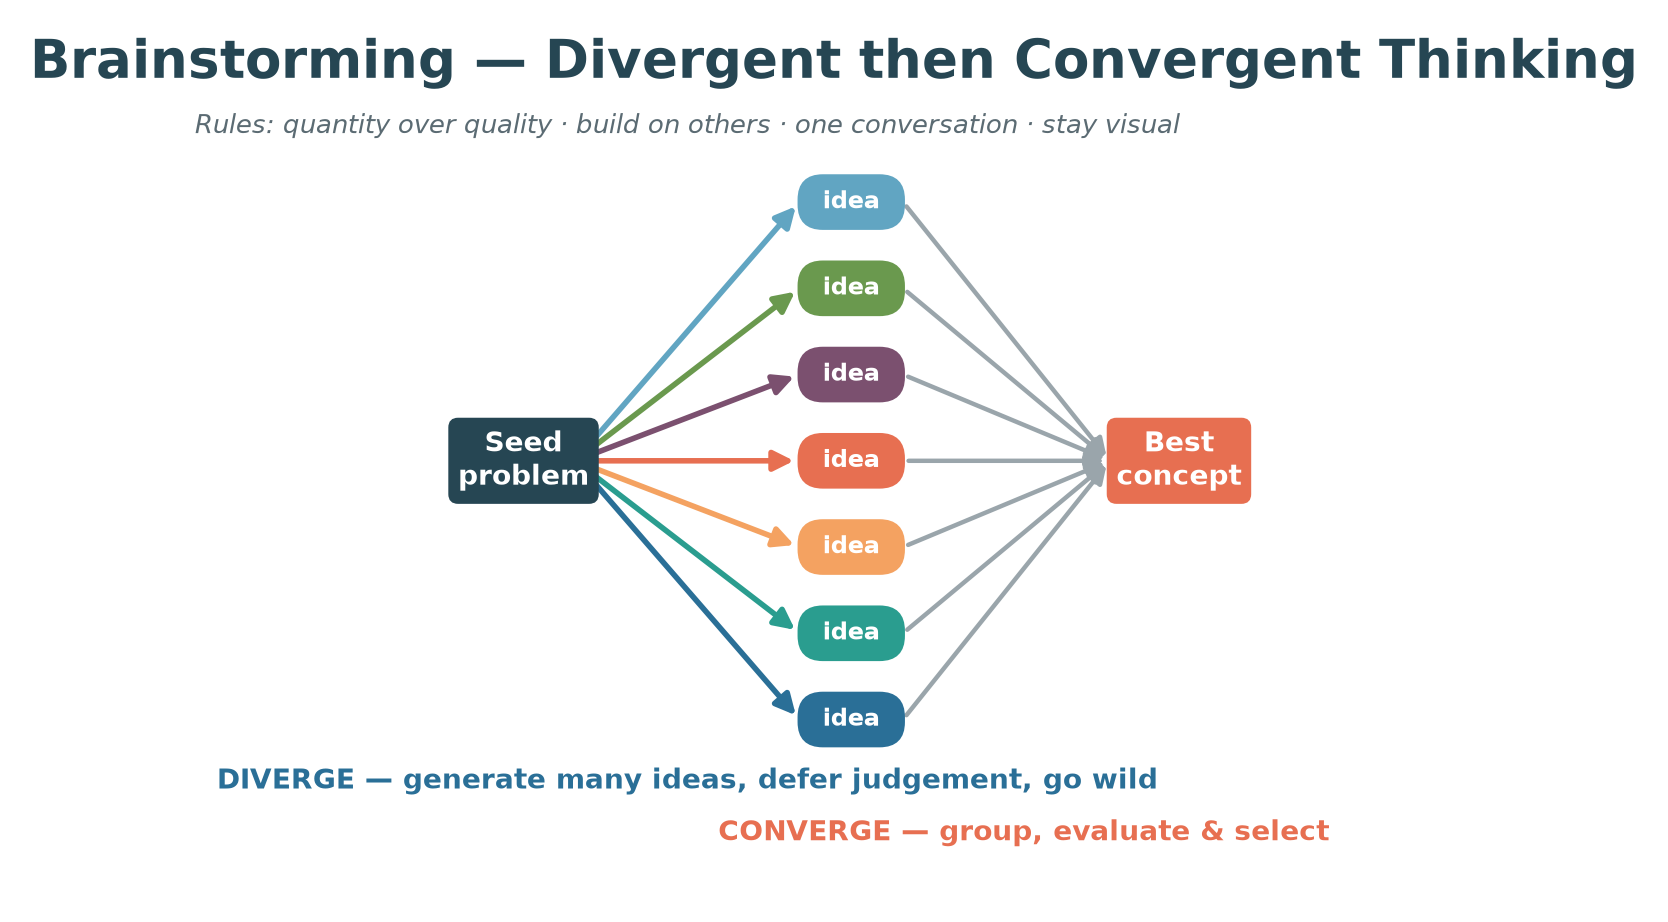
\includegraphics[width=\linewidth]{figures/divergent_convergent.png}
    \end{column}
    \begin{column}{0.42\textwidth}\scriptsize
      Creative work alternates two modes:
      \begin{itemize}\scriptsize
        \item \pill{dtblue}{Diverge} — generate many ideas, defer judgement.
        \item \pill{dtcoral}{Converge} — group, evaluate \& select.
      \end{itemize}
      \vspace{0.3em}
      \textbf{Brainstorming rules}
      \begin{itemize}\scriptsize
        \item Go for quantity.
        \item Build on others' ideas.
        \item One conversation at a time.
        \item Stay visual; welcome wild ideas.
      \end{itemize}
    \end{column}
  \end{columns}
\end{frame}

\begin{frame}{The Five Stages of Design Thinking}
  \bigfig{dt_process.png}{Empathize $\to$ Define $\to$ Ideate $\to$ Prototype $\to$ Test — iterative, not linear.}
\end{frame}

\begin{frame}{Stages in Detail (1--3)}
  \accentrule\\[0.3em]
  \small
  \begin{description}\small
    \item[\textcolor{dtblue}{1. Empathize}] Observe and engage with users;
      conduct interviews and immerse yourself in their world. \emph{Example:}
      shadowing commuters to learn how they use a ticket machine.
    \item[\textcolor{dtteal}{2. Define}] Synthesise observations into a clear,
      user-centred \kw{problem statement} (a Point-of-View). \emph{Example:}
      "Busy commuters need a faster way to buy tickets because queues cause
      stress."
    \item[\textcolor{dtyellow}{3. Ideate}] Generate a wide range of ideas
      through brainstorming, sketching and mind-mapping — \emph{quantity over
      quality} first.
  \end{description}
\end{frame}

\begin{frame}{Stages in Detail (4--5)}
  \accentrule\\[0.3em]
  \small
  \begin{description}\small
    \item[\textcolor{dtorange}{4. Prototype}] Build quick, inexpensive,
      scaled-down versions to explore ideas. \emph{Example:} a paper mock-up of
      the ticket-machine screen.
    \item[\textcolor{dtcoral}{5. Test}] Try prototypes with real users, gather
      feedback and refine. Testing often \emph{re-defines the problem} —
      sending you back to earlier stages.
  \end{description}
  \vspace{0.3em}
  \begin{block}{Being ingenious}\scriptsize
    The stages are a \emph{flexible toolkit}, not a rigid recipe. Teams loop,
    skip and revisit stages as they learn.
  \end{block}
\end{frame}

\begin{frame}{The Double Diamond}
  \begin{columns}[c]
    \begin{column}{0.62\textwidth}
      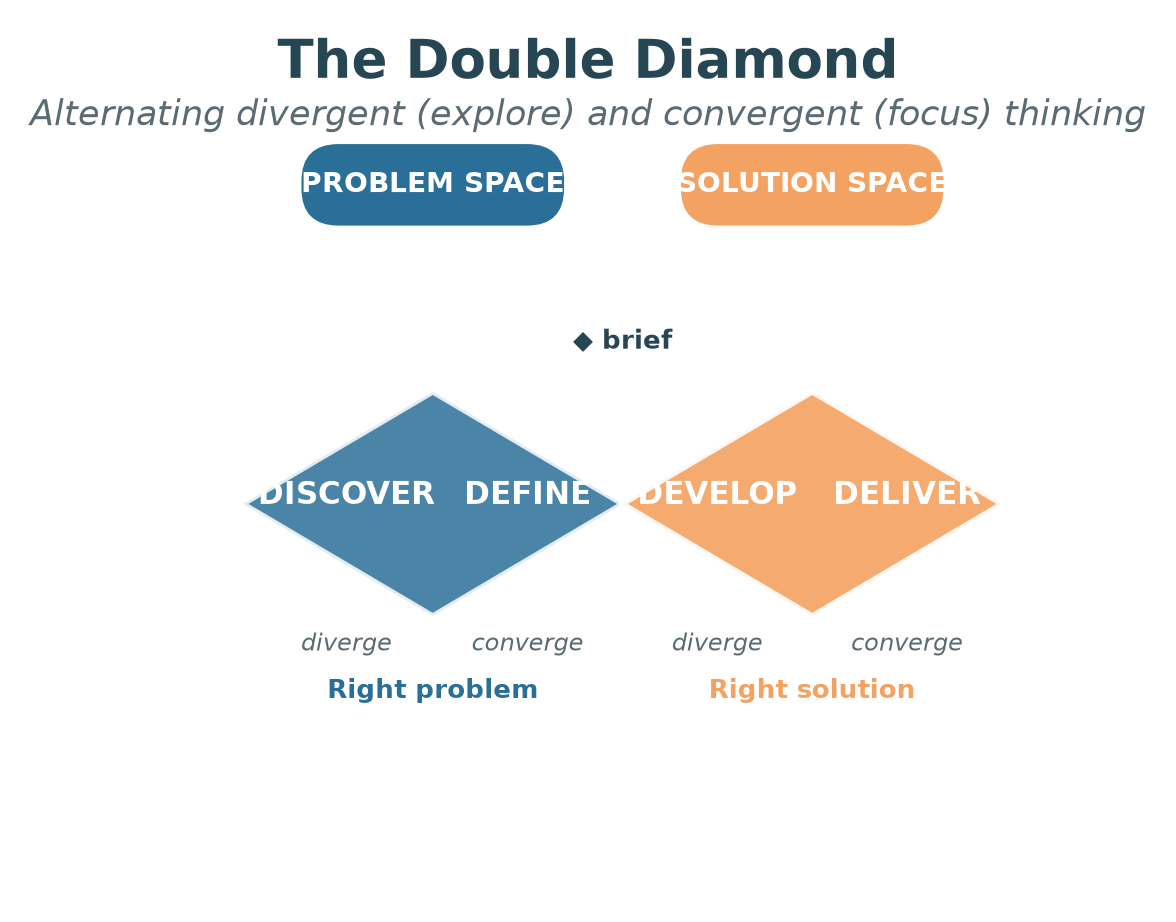
\includegraphics[width=\linewidth]{figures/double_diamond.png}
    \end{column}
    \begin{column}{0.38\textwidth}\scriptsize
      A popular map of the design process:
      \begin{itemize}\scriptsize
        \item \pill{dtblue}{Discover \& Define} — find the \emph{right problem}.
        \item \pill{dtorange}{Develop \& Deliver} — build the \emph{right
              solution}.
      \end{itemize}
      \vspace{0.3em}
      Each diamond widens (diverge) then narrows (converge).
    \end{column}
  \end{columns}
\end{frame}

\begin{frame}{Creative Thinking \& Problem Solving}
  \begin{columns}[c]
    \begin{column}{0.6\textwidth}
      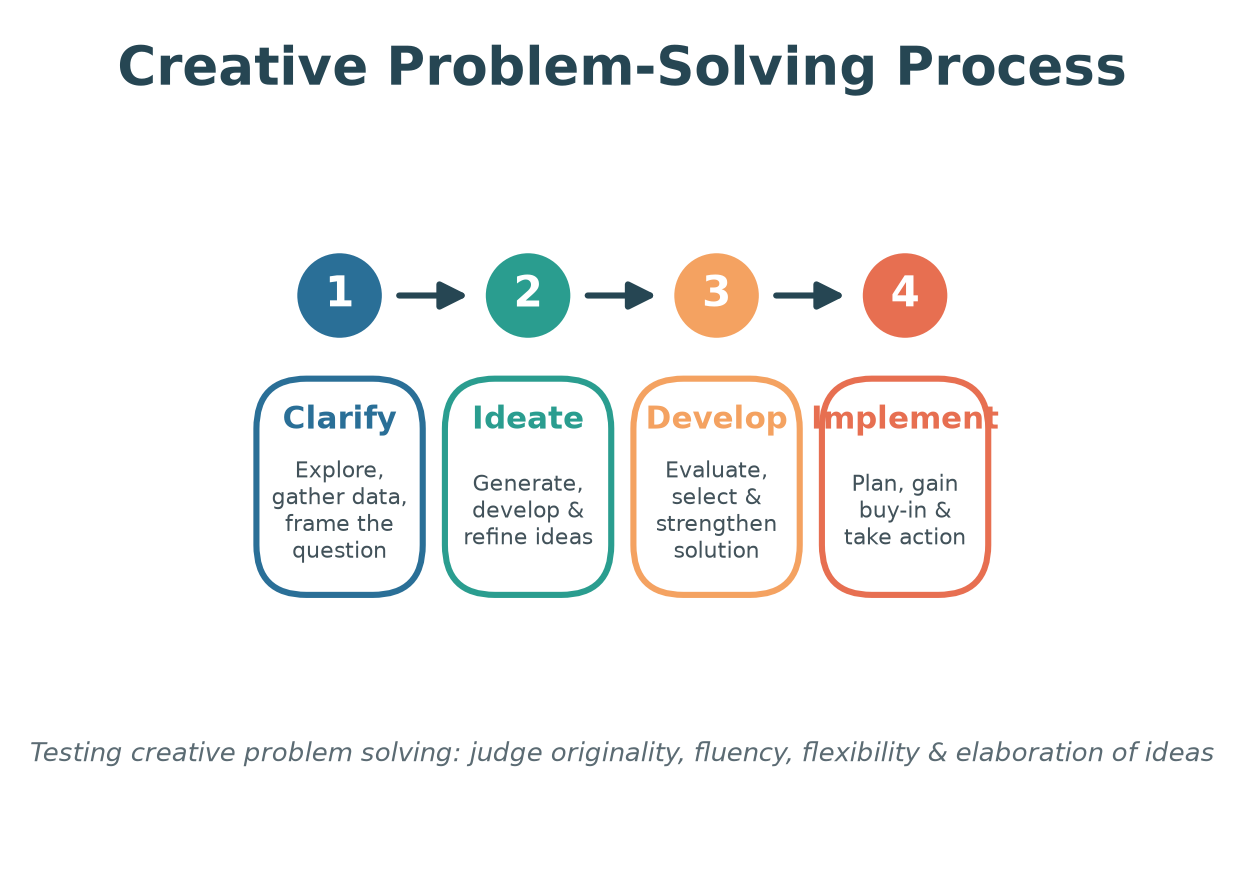
\includegraphics[width=\linewidth]{figures/creative_problem_solving.png}
    \end{column}
    \begin{column}{0.4\textwidth}\scriptsize
      Creative problem solving moves through four stages: \kwt{Clarify},
      \kwt{Ideate}, \kwt{Develop} and \kwt{Implement}.
      \vspace{0.4em}
      \textbf{Testing creative problem solving} — judge ideas on:
      \begin{itemize}\scriptsize
        \item \emph{Fluency} — number of ideas.
        \item \emph{Flexibility} — variety of ideas.
        \item \emph{Originality} — novelty.
        \item \emph{Elaboration} — detail \& refinement.
      \end{itemize}
    \end{column}
  \end{columns}
\end{frame}

%% Requires the macros/colours defined in main.tex's preamble.

%==============================================================================
\section{Basics of Design Thinking}
%==============================================================================
\unitdivider{II}{Basics of Design Thinking}{The mindset, the process, the tools}

\begin{frame}{What is Design Thinking?}
  \accentrule\\[0.3em]
  \begin{columns}[T]
    \begin{column}{0.55\textwidth}\small
      \begin{block}{Definition}\small
        A \kw{human-centred}, iterative problem-solving approach that seeks
        to understand users, challenge assumptions, redefine problems and
        create innovative solutions to prototype and test.
      \end{block}
      \textbf{Need for design thinking}
      \begin{itemize}\small
        \item Problems are \kwc{complex \& ill-defined}.
        \item Users' real needs are often \emph{hidden}.
        \item Reduces the risk of building the wrong thing.
      \end{itemize}
    \end{column}
    \begin{column}{0.45\textwidth}\small
      \textbf{Objectives}
      \begin{itemize}\small
        \item Keep the \kwt{user at the centre}.
        \item Encourage \kwt{creativity \& collaboration}.
        \item \kwt{Fail early}, learn cheaply.
        \item Turn insight into tangible value.
      \end{itemize}
    \end{column}
  \end{columns}
\end{frame}

\begin{frame}{Concepts \& Brainstorming}
  \begin{columns}[c]
    \begin{column}{0.58\textwidth}
      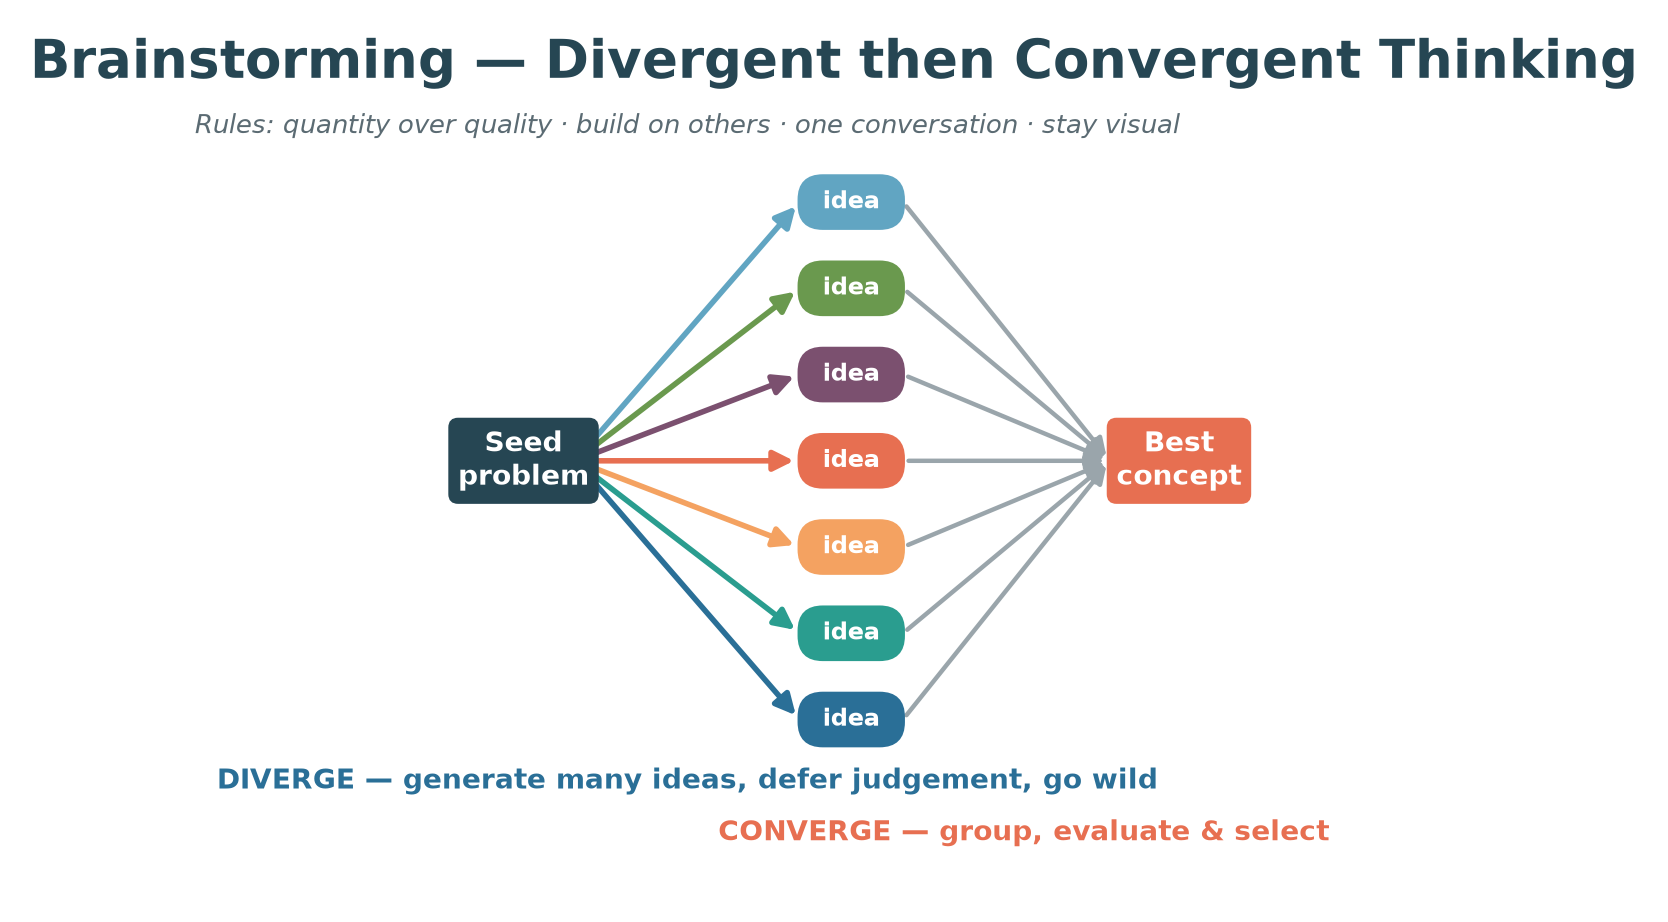
\includegraphics[width=\linewidth]{figures/divergent_convergent.png}
    \end{column}
    \begin{column}{0.42\textwidth}\scriptsize
      Creative work alternates two modes:
      \begin{itemize}\scriptsize
        \item \pill{dtblue}{Diverge} — generate many ideas, defer judgement.
        \item \pill{dtcoral}{Converge} — group, evaluate \& select.
      \end{itemize}
      \vspace{0.3em}
      \textbf{Brainstorming rules}
      \begin{itemize}\scriptsize
        \item Go for quantity.
        \item Build on others' ideas.
        \item One conversation at a time.
        \item Stay visual; welcome wild ideas.
      \end{itemize}
    \end{column}
  \end{columns}
\end{frame}

\begin{frame}{The Five Stages of Design Thinking}
  \bigfig{dt_process.png}{Empathize $\to$ Define $\to$ Ideate $\to$ Prototype $\to$ Test — iterative, not linear.}
\end{frame}

\begin{frame}{Stages in Detail (1--3)}
  \accentrule\\[0.3em]
  \small
  \begin{description}\small
    \item[\textcolor{dtblue}{1. Empathize}] Observe and engage with users;
      conduct interviews and immerse yourself in their world. \emph{Example:}
      shadowing commuters to learn how they use a ticket machine.
    \item[\textcolor{dtteal}{2. Define}] Synthesise observations into a clear,
      user-centred \kw{problem statement} (a Point-of-View). \emph{Example:}
      "Busy commuters need a faster way to buy tickets because queues cause
      stress."
    \item[\textcolor{dtyellow}{3. Ideate}] Generate a wide range of ideas
      through brainstorming, sketching and mind-mapping — \emph{quantity over
      quality} first.
  \end{description}
\end{frame}

\begin{frame}{Stages in Detail (4--5)}
  \accentrule\\[0.3em]
  \small
  \begin{description}\small
    \item[\textcolor{dtorange}{4. Prototype}] Build quick, inexpensive,
      scaled-down versions to explore ideas. \emph{Example:} a paper mock-up of
      the ticket-machine screen.
    \item[\textcolor{dtcoral}{5. Test}] Try prototypes with real users, gather
      feedback and refine. Testing often \emph{re-defines the problem} —
      sending you back to earlier stages.
  \end{description}
  \vspace{0.3em}
  \begin{block}{Being ingenious}\scriptsize
    The stages are a \emph{flexible toolkit}, not a rigid recipe. Teams loop,
    skip and revisit stages as they learn.
  \end{block}
\end{frame}

\begin{frame}{The Double Diamond}
  \begin{columns}[c]
    \begin{column}{0.62\textwidth}
      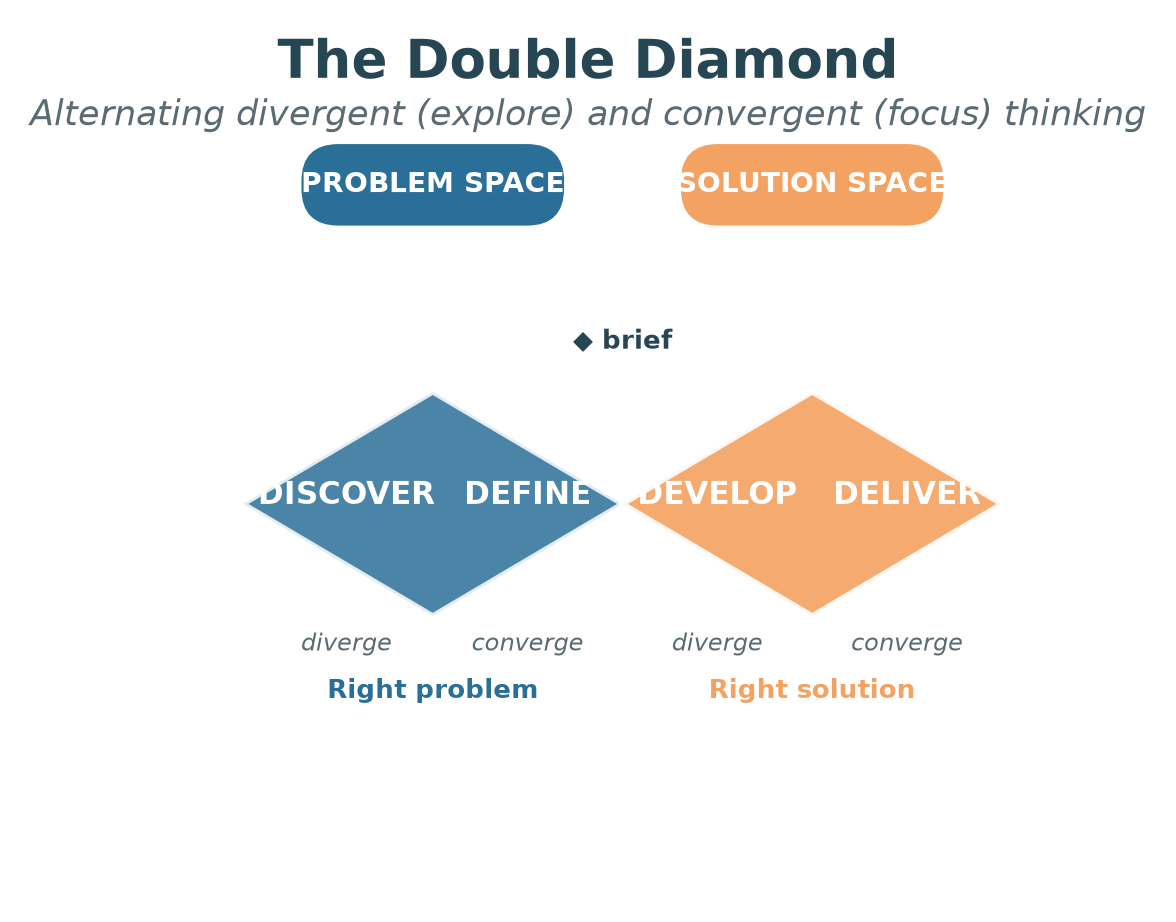
\includegraphics[width=\linewidth]{figures/double_diamond.png}
    \end{column}
    \begin{column}{0.38\textwidth}\scriptsize
      A popular map of the design process:
      \begin{itemize}\scriptsize
        \item \pill{dtblue}{Discover \& Define} — find the \emph{right problem}.
        \item \pill{dtorange}{Develop \& Deliver} — build the \emph{right
              solution}.
      \end{itemize}
      \vspace{0.3em}
      Each diamond widens (diverge) then narrows (converge).
    \end{column}
  \end{columns}
\end{frame}

\begin{frame}{Creative Thinking \& Problem Solving}
  \begin{columns}[c]
    \begin{column}{0.6\textwidth}
      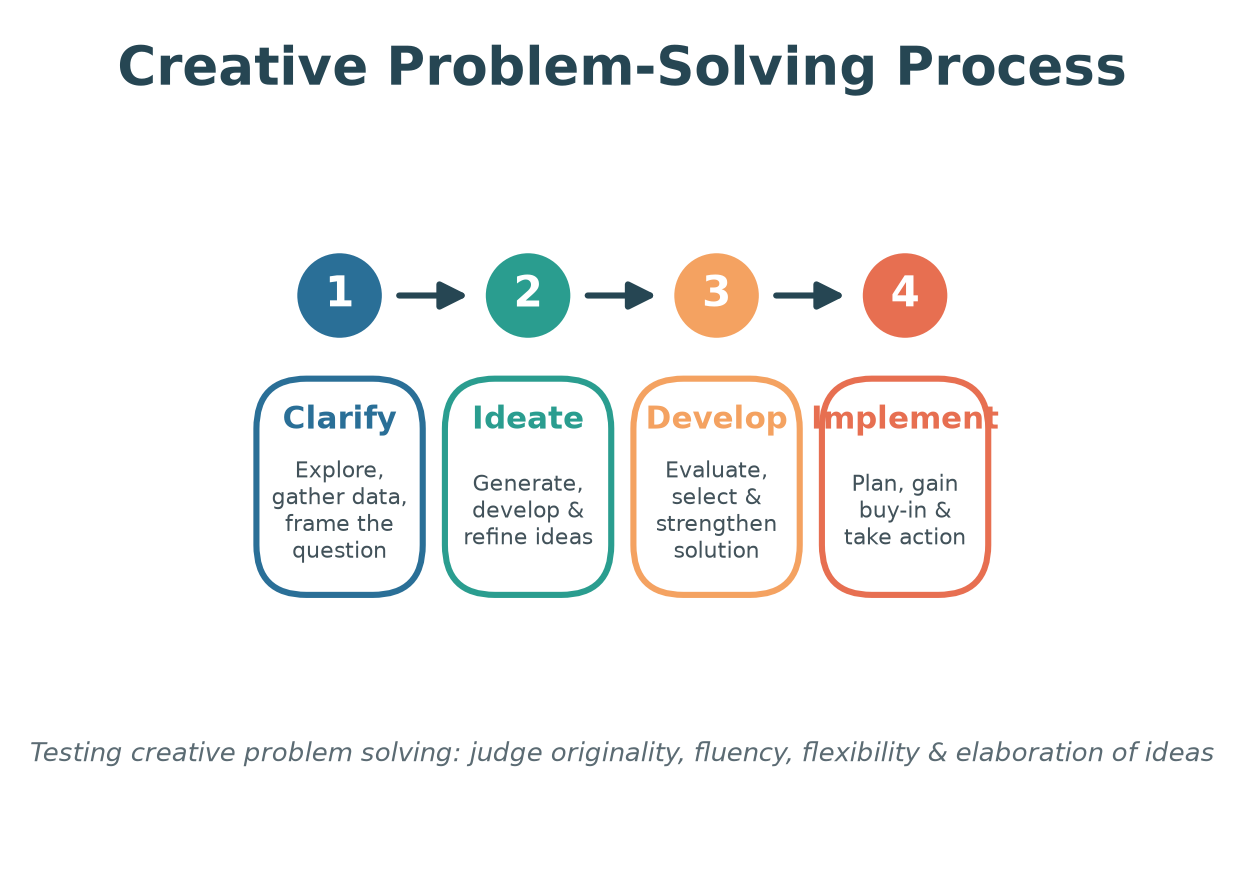
\includegraphics[width=\linewidth]{figures/creative_problem_solving.png}
    \end{column}
    \begin{column}{0.4\textwidth}\scriptsize
      Creative problem solving moves through four stages: \kwt{Clarify},
      \kwt{Ideate}, \kwt{Develop} and \kwt{Implement}.
      \vspace{0.4em}
      \textbf{Testing creative problem solving} — judge ideas on:
      \begin{itemize}\scriptsize
        \item \emph{Fluency} — number of ideas.
        \item \emph{Flexibility} — variety of ideas.
        \item \emph{Originality} — novelty.
        \item \emph{Elaboration} — detail \& refinement.
      \end{itemize}
    \end{column}
  \end{columns}
\end{frame}

%% Requires the macros/colours defined in main.tex's preamble.

%==============================================================================
\section{Basics of Design Thinking}
%==============================================================================
\unitdivider{II}{Basics of Design Thinking}{The mindset, the process, the tools}

\begin{frame}{What is Design Thinking?}
  \accentrule\\[0.3em]
  \begin{columns}[T]
    \begin{column}{0.55\textwidth}\small
      \begin{block}{Definition}\small
        A \kw{human-centred}, iterative problem-solving approach that seeks
        to understand users, challenge assumptions, redefine problems and
        create innovative solutions to prototype and test.
      \end{block}
      \textbf{Need for design thinking}
      \begin{itemize}\small
        \item Problems are \kwc{complex \& ill-defined}.
        \item Users' real needs are often \emph{hidden}.
        \item Reduces the risk of building the wrong thing.
      \end{itemize}
    \end{column}
    \begin{column}{0.45\textwidth}\small
      \textbf{Objectives}
      \begin{itemize}\small
        \item Keep the \kwt{user at the centre}.
        \item Encourage \kwt{creativity \& collaboration}.
        \item \kwt{Fail early}, learn cheaply.
        \item Turn insight into tangible value.
      \end{itemize}
    \end{column}
  \end{columns}
\end{frame}

\begin{frame}{Concepts \& Brainstorming}
  \begin{columns}[c]
    \begin{column}{0.58\textwidth}
      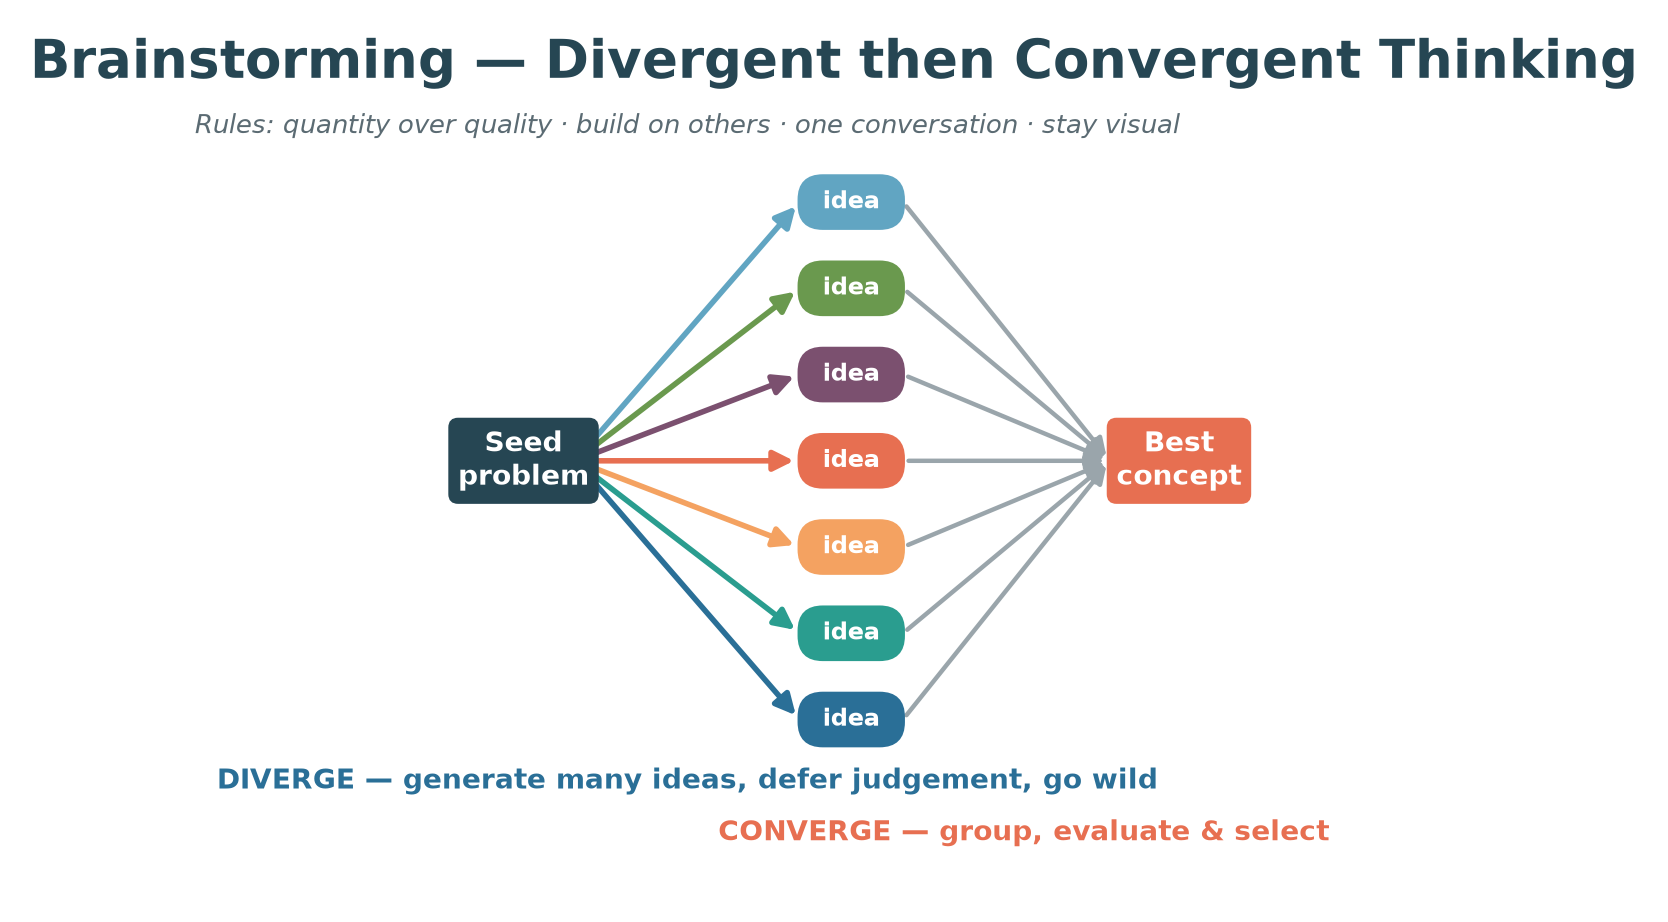
\includegraphics[width=\linewidth]{figures/divergent_convergent.png}
    \end{column}
    \begin{column}{0.42\textwidth}\scriptsize
      Creative work alternates two modes:
      \begin{itemize}\scriptsize
        \item \pill{dtblue}{Diverge} — generate many ideas, defer judgement.
        \item \pill{dtcoral}{Converge} — group, evaluate \& select.
      \end{itemize}
      \vspace{0.3em}
      \textbf{Brainstorming rules}
      \begin{itemize}\scriptsize
        \item Go for quantity.
        \item Build on others' ideas.
        \item One conversation at a time.
        \item Stay visual; welcome wild ideas.
      \end{itemize}
    \end{column}
  \end{columns}
\end{frame}

\begin{frame}{The Five Stages of Design Thinking}
  \bigfig{dt_process.png}{Empathize $\to$ Define $\to$ Ideate $\to$ Prototype $\to$ Test — iterative, not linear.}
\end{frame}

\begin{frame}{Stages in Detail (1--3)}
  \accentrule\\[0.3em]
  \small
  \begin{description}\small
    \item[\textcolor{dtblue}{1. Empathize}] Observe and engage with users;
      conduct interviews and immerse yourself in their world. \emph{Example:}
      shadowing commuters to learn how they use a ticket machine.
    \item[\textcolor{dtteal}{2. Define}] Synthesise observations into a clear,
      user-centred \kw{problem statement} (a Point-of-View). \emph{Example:}
      "Busy commuters need a faster way to buy tickets because queues cause
      stress."
    \item[\textcolor{dtyellow}{3. Ideate}] Generate a wide range of ideas
      through brainstorming, sketching and mind-mapping — \emph{quantity over
      quality} first.
  \end{description}
\end{frame}

\begin{frame}{Stages in Detail (4--5)}
  \accentrule\\[0.3em]
  \small
  \begin{description}\small
    \item[\textcolor{dtorange}{4. Prototype}] Build quick, inexpensive,
      scaled-down versions to explore ideas. \emph{Example:} a paper mock-up of
      the ticket-machine screen.
    \item[\textcolor{dtcoral}{5. Test}] Try prototypes with real users, gather
      feedback and refine. Testing often \emph{re-defines the problem} —
      sending you back to earlier stages.
  \end{description}
  \vspace{0.3em}
  \begin{block}{Being ingenious}\scriptsize
    The stages are a \emph{flexible toolkit}, not a rigid recipe. Teams loop,
    skip and revisit stages as they learn.
  \end{block}
\end{frame}

\begin{frame}{The Double Diamond}
  \begin{columns}[c]
    \begin{column}{0.62\textwidth}
      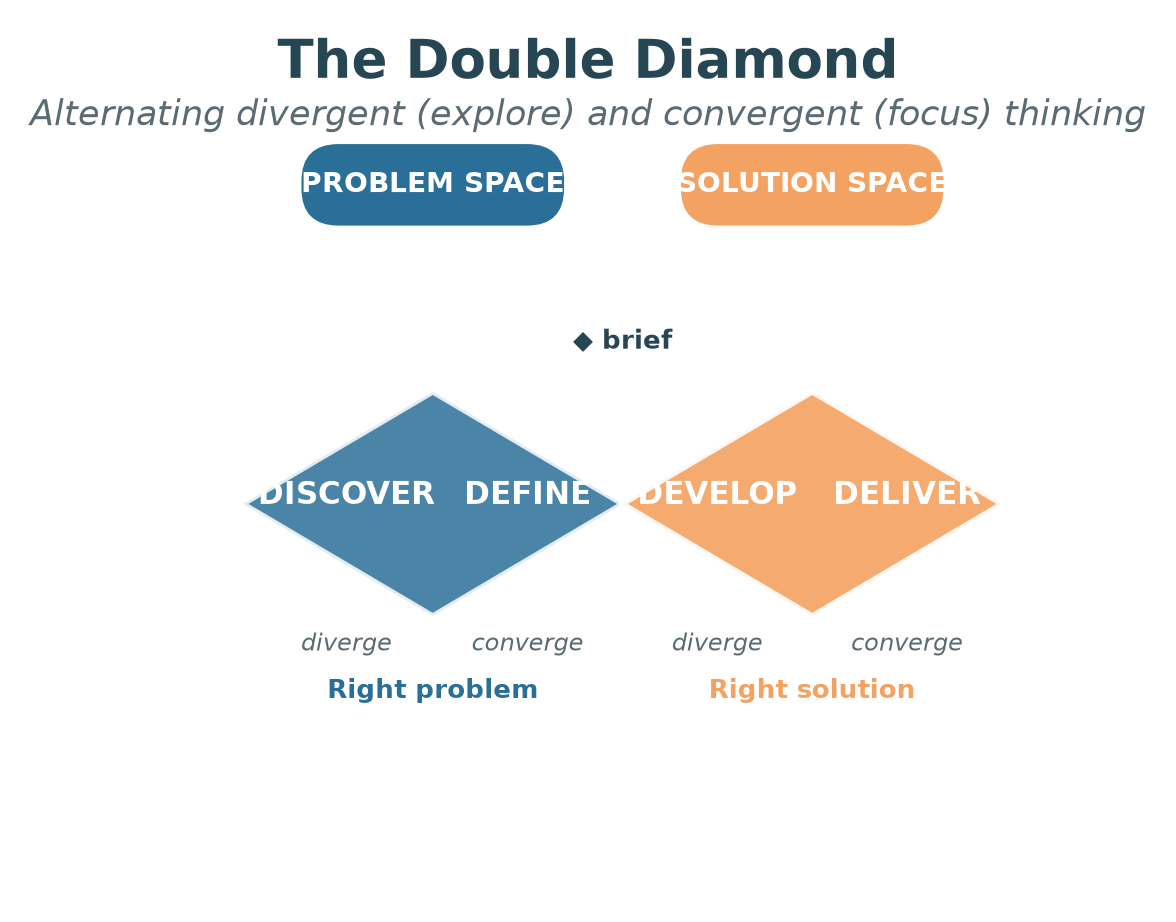
\includegraphics[width=\linewidth]{figures/double_diamond.png}
    \end{column}
    \begin{column}{0.38\textwidth}\scriptsize
      A popular map of the design process:
      \begin{itemize}\scriptsize
        \item \pill{dtblue}{Discover \& Define} — find the \emph{right problem}.
        \item \pill{dtorange}{Develop \& Deliver} — build the \emph{right
              solution}.
      \end{itemize}
      \vspace{0.3em}
      Each diamond widens (diverge) then narrows (converge).
    \end{column}
  \end{columns}
\end{frame}

\begin{frame}{Creative Thinking \& Problem Solving}
  \begin{columns}[c]
    \begin{column}{0.6\textwidth}
      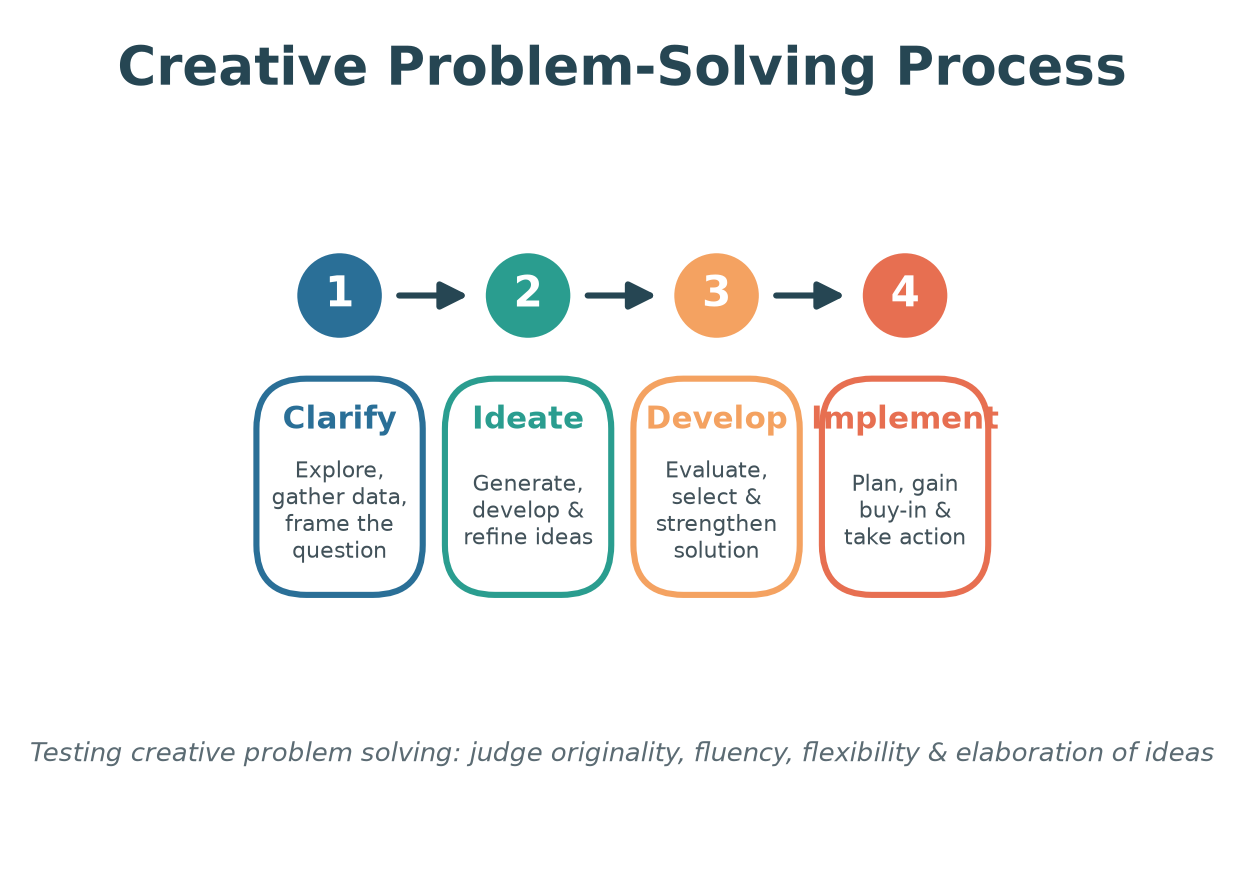
\includegraphics[width=\linewidth]{figures/creative_problem_solving.png}
    \end{column}
    \begin{column}{0.4\textwidth}\scriptsize
      Creative problem solving moves through four stages: \kwt{Clarify},
      \kwt{Ideate}, \kwt{Develop} and \kwt{Implement}.
      \vspace{0.4em}
      \textbf{Testing creative problem solving} — judge ideas on:
      \begin{itemize}\scriptsize
        \item \emph{Fluency} — number of ideas.
        \item \emph{Flexibility} — variety of ideas.
        \item \emph{Originality} — novelty.
        \item \emph{Elaboration} — detail \& refinement.
      \end{itemize}
    \end{column}
  \end{columns}
\end{frame}

%% Requires the macros/colours defined in main.tex's preamble.

%==============================================================================
\section{Basics of Design Thinking}
%==============================================================================
\unitdivider{II}{Basics of Design Thinking}{The mindset, the process, the tools}

\begin{frame}{What is Design Thinking?}
  \accentrule\\[0.3em]
  \begin{columns}[T]
    \begin{column}{0.55\textwidth}\small
      \begin{block}{Definition}\small
        A \kw{human-centred}, iterative problem-solving approach that seeks
        to understand users, challenge assumptions, redefine problems and
        create innovative solutions to prototype and test.
      \end{block}
      \textbf{Need for design thinking}
      \begin{itemize}\small
        \item Problems are \kwc{complex \& ill-defined}.
        \item Users' real needs are often \emph{hidden}.
        \item Reduces the risk of building the wrong thing.
      \end{itemize}
    \end{column}
    \begin{column}{0.45\textwidth}\small
      \textbf{Objectives}
      \begin{itemize}\small
        \item Keep the \kwt{user at the centre}.
        \item Encourage \kwt{creativity \& collaboration}.
        \item \kwt{Fail early}, learn cheaply.
        \item Turn insight into tangible value.
      \end{itemize}
    \end{column}
  \end{columns}
\end{frame}

\begin{frame}{Concepts \& Brainstorming}
  \begin{columns}[c]
    \begin{column}{0.58\textwidth}
      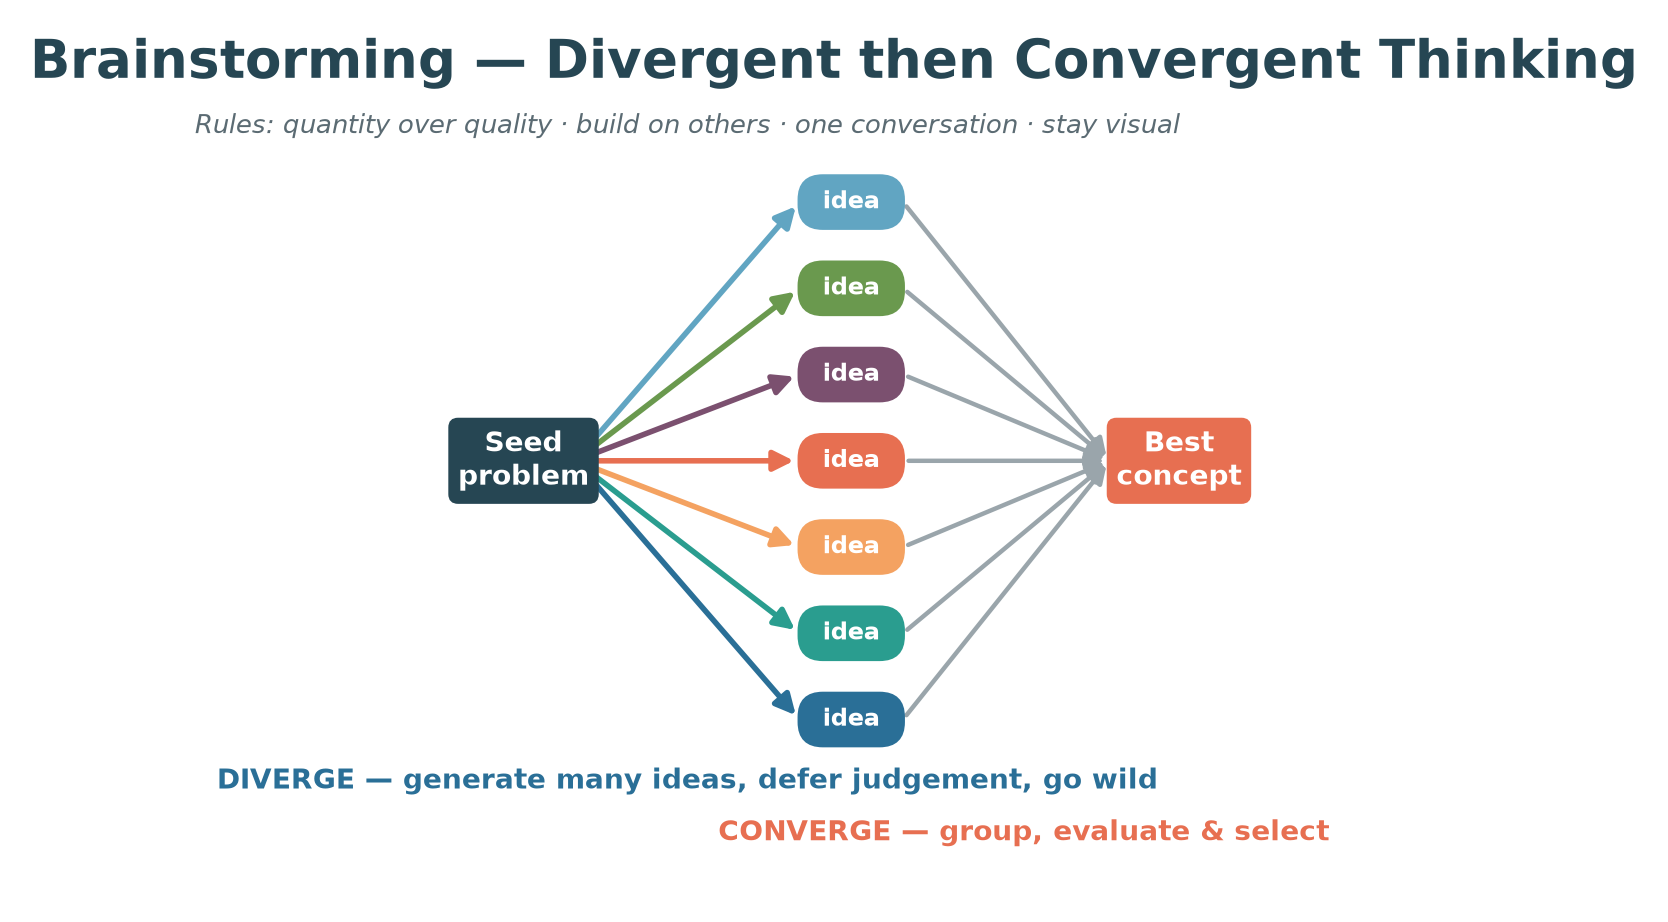
\includegraphics[width=\linewidth]{figures/divergent_convergent.png}
    \end{column}
    \begin{column}{0.42\textwidth}\scriptsize
      Creative work alternates two modes:
      \begin{itemize}\scriptsize
        \item \pill{dtblue}{Diverge} — generate many ideas, defer judgement.
        \item \pill{dtcoral}{Converge} — group, evaluate \& select.
      \end{itemize}
      \vspace{0.3em}
      \textbf{Brainstorming rules}
      \begin{itemize}\scriptsize
        \item Go for quantity.
        \item Build on others' ideas.
        \item One conversation at a time.
        \item Stay visual; welcome wild ideas.
      \end{itemize}
    \end{column}
  \end{columns}
\end{frame}

\begin{frame}{The Five Stages of Design Thinking}
  \bigfig{dt_process.png}{Empathize $\to$ Define $\to$ Ideate $\to$ Prototype $\to$ Test — iterative, not linear.}
\end{frame}

\begin{frame}{Stages in Detail (1--3)}
  \accentrule\\[0.3em]
  \small
  \begin{description}\small
    \item[\textcolor{dtblue}{1. Empathize}] Observe and engage with users;
      conduct interviews and immerse yourself in their world. \emph{Example:}
      shadowing commuters to learn how they use a ticket machine.
    \item[\textcolor{dtteal}{2. Define}] Synthesise observations into a clear,
      user-centred \kw{problem statement} (a Point-of-View). \emph{Example:}
      "Busy commuters need a faster way to buy tickets because queues cause
      stress."
    \item[\textcolor{dtyellow}{3. Ideate}] Generate a wide range of ideas
      through brainstorming, sketching and mind-mapping — \emph{quantity over
      quality} first.
  \end{description}
\end{frame}

\begin{frame}{Stages in Detail (4--5)}
  \accentrule\\[0.3em]
  \small
  \begin{description}\small
    \item[\textcolor{dtorange}{4. Prototype}] Build quick, inexpensive,
      scaled-down versions to explore ideas. \emph{Example:} a paper mock-up of
      the ticket-machine screen.
    \item[\textcolor{dtcoral}{5. Test}] Try prototypes with real users, gather
      feedback and refine. Testing often \emph{re-defines the problem} —
      sending you back to earlier stages.
  \end{description}
  \vspace{0.3em}
  \begin{block}{Being ingenious}\scriptsize
    The stages are a \emph{flexible toolkit}, not a rigid recipe. Teams loop,
    skip and revisit stages as they learn.
  \end{block}
\end{frame}

\begin{frame}{The Double Diamond}
  \begin{columns}[c]
    \begin{column}{0.62\textwidth}
      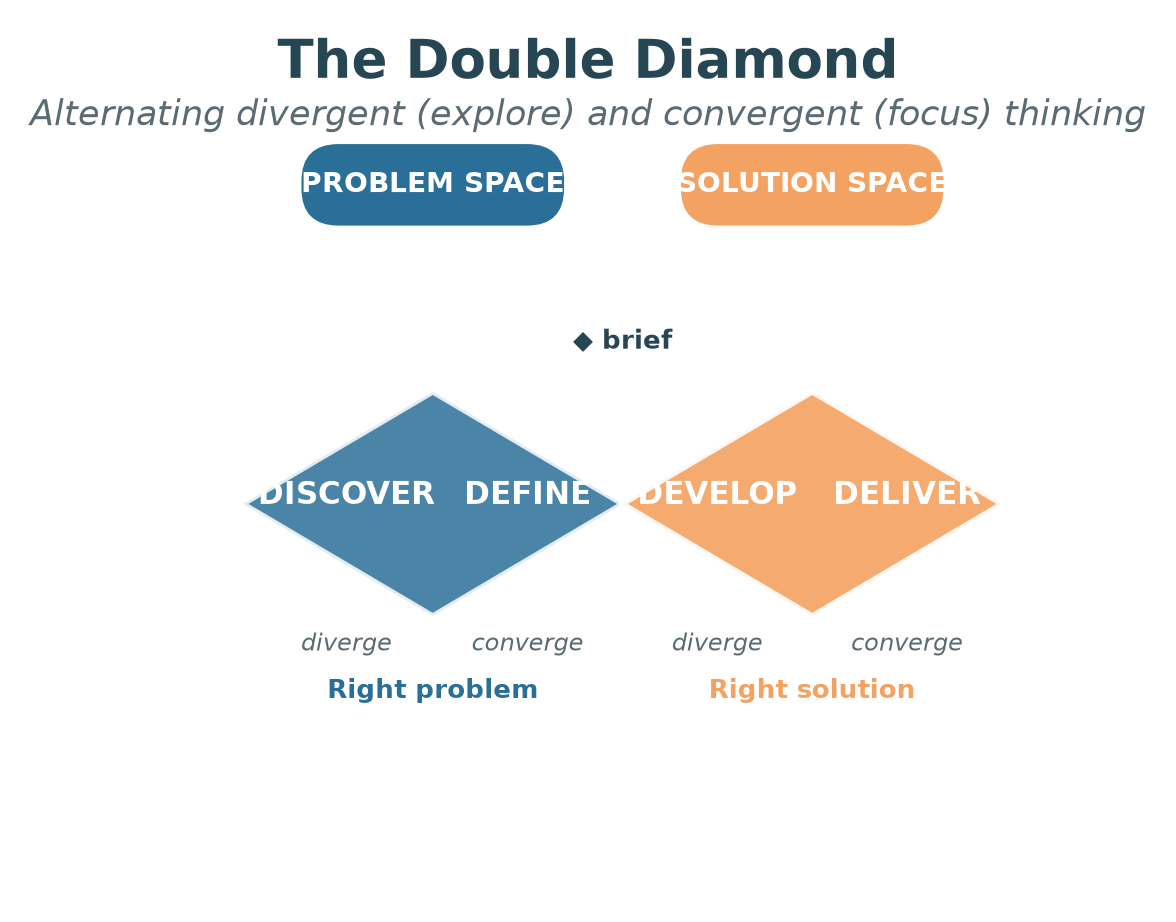
\includegraphics[width=\linewidth]{figures/double_diamond.png}
    \end{column}
    \begin{column}{0.38\textwidth}\scriptsize
      A popular map of the design process:
      \begin{itemize}\scriptsize
        \item \pill{dtblue}{Discover \& Define} — find the \emph{right problem}.
        \item \pill{dtorange}{Develop \& Deliver} — build the \emph{right
              solution}.
      \end{itemize}
      \vspace{0.3em}
      Each diamond widens (diverge) then narrows (converge).
    \end{column}
  \end{columns}
\end{frame}

\begin{frame}{Creative Thinking \& Problem Solving}
  \begin{columns}[c]
    \begin{column}{0.6\textwidth}
      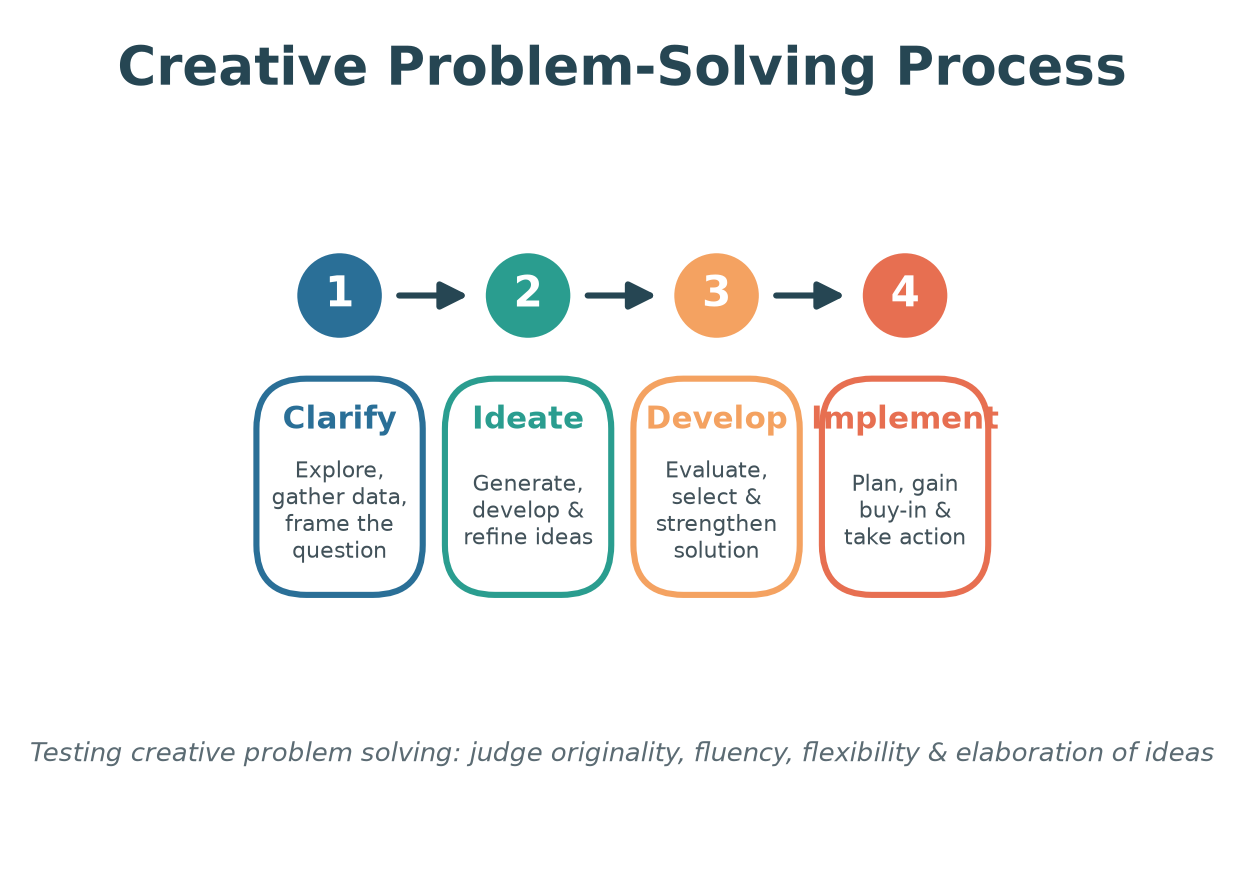
\includegraphics[width=\linewidth]{figures/creative_problem_solving.png}
    \end{column}
    \begin{column}{0.4\textwidth}\scriptsize
      Creative problem solving moves through four stages: \kwt{Clarify},
      \kwt{Ideate}, \kwt{Develop} and \kwt{Implement}.
      \vspace{0.4em}
      \textbf{Testing creative problem solving} — judge ideas on:
      \begin{itemize}\scriptsize
        \item \emph{Fluency} — number of ideas.
        \item \emph{Flexibility} — variety of ideas.
        \item \emph{Originality} — novelty.
        \item \emph{Elaboration} — detail \& refinement.
      \end{itemize}
    \end{column}
  \end{columns}
\end{frame}
